\chapter{Appliance Recognition }

Appliance recognition and load disaggregation is some of the key aspects in \ab{NILM}[non intrusive load monitoring]. The main purpose of the \ab{NILM} approach is to better understand the power usage in the home, and help the different households to more optimal power savings. This is done by informing the residents about the power consumption of individual appliances. It is shown that informing a household about its usages pattern can lead to significant savings \citep{RefWorks:33}. This makes the basis for load disaggregation, where appliance specific load is guessed based on the main meter load. This enables the user to know what uses the energy and when.

One other aspect of \ab{NILM} is event detection. Sometime the actual consumption of an appliance is not as important as when it was used, and for how long. This is a simpler task than guessing the true consumption, and is for some applications a better approach. As an example is this kind of information sufficient if we want to track the activity of a elderly person in a assisted living situation. 

\section{NILM Concepts And Challenges} 
The aim of \ab{NILM} is to partition the hole house consumption data in to appliance specific consumption. 
\begin{equation}
	P(t) = p_1(t) + p_2(t) + ... + p_n(t)
	\label{EQ:PAC}
\end{equation}
This can be seen as in equation \ref{EQ:PAC} where $P(t)$ is the total consumption at time $t$, and $p_n(t)$ is the consumption of appliance $n$ at time $t$. The aim is to partition $P(t)$ back to the different appliance specific consumptions. In order to structure the problem we categorise the appliances in 4 groups\citep{RefWorks:17} 

\begin{tabularx}{\linewidth}{ r X }
Type-I:&Appliances that only have 2 states corresponding to on/off. This could be a lamp or a water boiler. \\
\\
Type-II:&These are appliances with multiple states, and can be modelled as a finite state machine. Many modern devices such as TV's, computers and washing machines fall in this category.   \\
\end{tabularx}

\begin{tabularx}{\linewidth}{ r X }
Type-III:&These appliances is referred to as "Continuously Variable
Devices". These devices have a variable power draw and is impossible to model as a finite state machine. This could be appliances like power drills, and dimmer lights. These are by far the hardest for the \ab{NILM} algorithms to detect. \\
\\
Type-IV:& These are a special kind of appliances that are always on and consume energy at a constant rate. Such devices could be smoke detectors and TV receivers.  \\
\end{tabularx}

Some of the different appliance types is illustrated on figure \ref{fig:ATO}. 


\begin{figure}[H]
\centering
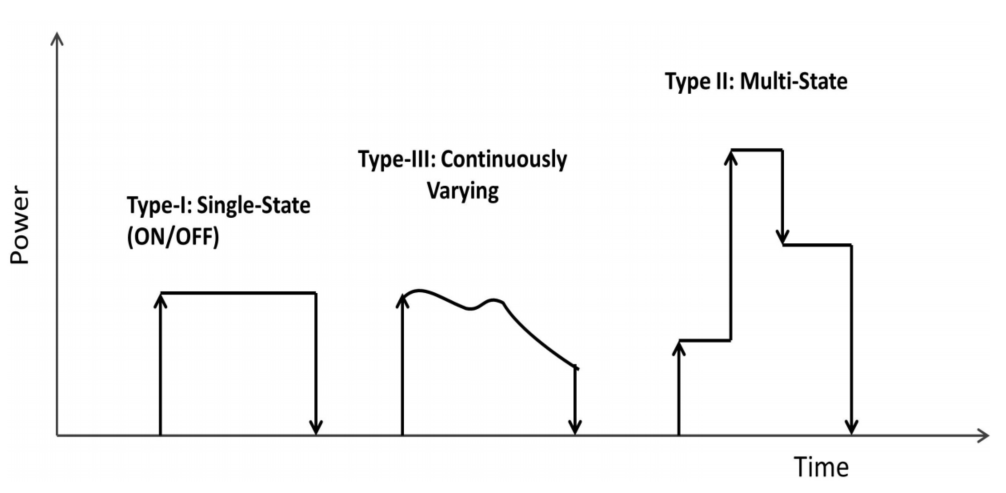
\includegraphics[width=0.6\textwidth]{billeder/Types.png}
\caption{Appliance types. Source \citep{RefWorks:17}}
\label{fig:ATO}
\end{figure}

The appliances in Type-IV is not a particular researched area, since it does not give the user much information to calculate savings from. These appliances is often using very little energy, and must not be turn off at will. 

Type-I and Type-II are very used, and can cover all most any appliance. In the area of event detection are the most common approach to see all appliances as Type-I appliances and detecting on/off events. Most appliances today is Type-II appliances due to growing amount of complicated electronics that are embedded in them. Then there are devices that are Type-II but most of the time act like Type-I appliances. An example of this is the vacuum cleaner. On most vacuum cleaners you are able to change the suction intensity, which makes it type two. But most people don't change this very often, so the energy usage looks more like a Type-I appliance. 
 
\subsection{NILM Features} 
For data disaggregation it is common to use method based on machine learning and optimization. The approach is to first extract features from the dataset, and then train or validate by using this features. 

In \ab{NILM} the features can be sub categorised in steady state, transient state and non-Traditional features.  These categories can be further expanded as shown on figure \ref{fig:FTR}. 

\begin{figure}[H]
\centering
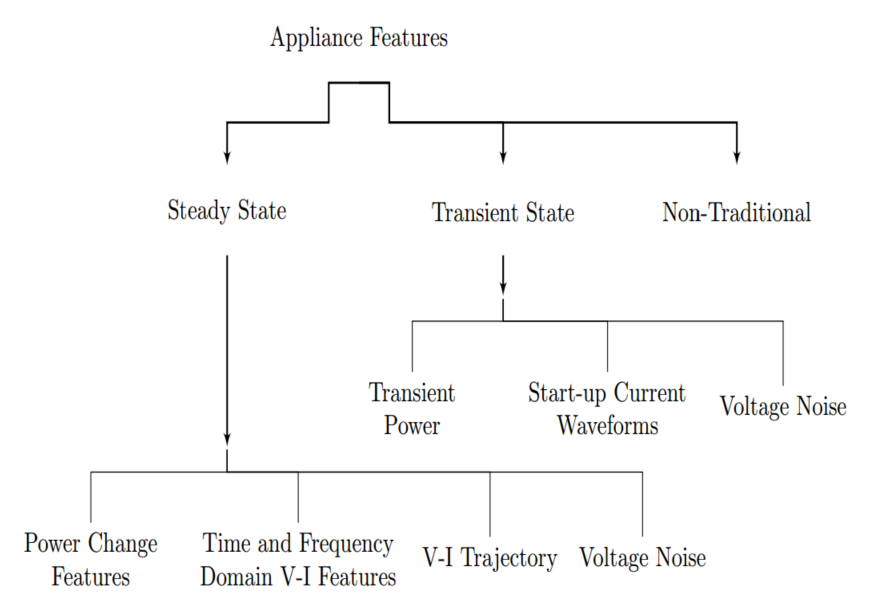
\includegraphics[width=0.6\textwidth]{billeder/featureOverview.png}
\caption{Feature types. Source \citep{RefWorks:17}}
\label{fig:FTR}
\end{figure}

Steady state features is features that can be extracted when the signal is in the stable state. Features that are often extracted in this state is "Power Change" which is the jump in power or reactive power usage. Time and frequency analysis is often used on the voltage and power signals of the meters. It is shown that analysing the harmonics in signals is a powerful way of making appliance detection \citep{RefWorks:29}.The trajectory between voltage and power usage is a god feature. This can be used to detect the reactive power of a signal, which is a give-away for inductive loads. Some researchers have shown that different appliances makes different noise profiles on the main line. Unfortunately does this kind of recognition require a extremely high sampling rate \citep{RefWorks:30}. 

The transient state of an appliance is a short state that comes when a appliance switches between steady states. In this state there often is appliance semi-unique waveforms in the current and voltage domain. The noise generated on the mainline in this state is also a good indication of the appliances type. 

There also exists a series of non-traditional features, that is used in special types of algorithms. One of them is based on matching the power usage profile to geometrical figures, and using the series of figures to recognize an appliance \citep{RefWorks:17}.  

Many of the above features requires a high sample rate in kHz or Mhz span in order to be effective. This kind of resolution is often not available since it is normal smart meters that are providing the data. For a smart meter a sample rate at 1 Hz would be considered fast, and for many applications this is down to $0.03$ Hz or slower. It is therefore common only to use the steady state features, and most of the time only the power change feature, which looks at changes in power, reactive power, current or voltage. 

\subsection{Learning Strategy} 
When you have extracted features from the signal there are several algorithms there can be selected for the training. They can roughly be split up in two categories optimization algorithms and pattern recognition algorithms. The optimization algorithms relies on a database of appliance info, and tries to find the subset of the database that are most likely to be in use. 

\begin{equation}
	M = \argmin_{x \in \powerset{D} } \left( \mid {\sum_{i = 0}^{I} x_i - \hat{y}  \mid} \right)
	\label{EQ:OMP}
\end{equation}

This is illustrated in equation \ref{EQ:OMP} were a set of appliances $M$ that correspond to the measured signal $\hat{y}$ needed to be found. This is achieved by searching the known database of all appliances $D$. This is done by taking the powerset of the database and finding the subset that minimises the error. This approach is fine for a small amounts of appliances, but for large databases and many appliances in use at the same time would this take far to long to be practical. 

Due to this, most researchers use pattern recognition techniques instead. These have the benefits of being more scalable, and be usable even if only parts of the device database is known. There are generality two approaches to pattern recognition: supervised and non-supervised. In supervised training it is assumed that the ground truth of your system is known. For a \ab{NILM} application this means that the true consumption of the appliance need to be available for the training process. This means that a sub meter must be placed to measure the appliances individually, which often is costly and time consuming. In non-supervised methods only the main meter readings are available, and no information about the appliances are known. This type of algorithms will usually try to cluster the readings in distinct groups cosponsoring to a guess of what appliances that correspond to the reading. Fore this kind of training it is easy to collect a big training set, but it requires the groups to be manually labelled afterwards.  
  
Most algorithms are based on clustering techniques and \ab{HMM}[hidden Markov models]. \Ab{HMM} have proven very effective when classifying Type-I and Type-II appliances. This is due to its ability to model state changes as a imported part of the classification. It is shown that using clustering techniques can greatly improve the classification, and reduce the training time. Artificial neural networks is also showing great promise, and is a topic that is currently in focus by many \ab{NILM} researchers. More on this in section \ref{sec:RecRelatedwork}. 

\subsection{NILM Challenges} 
There are many challenges in \ab{NILM}. One is the Type-III appliances. Due to there varying, and at time random, energy consumption it is hard to fit them to a behavioural model. This is made further harder by the low sample rate. Many great features of the appliances is hidden due to the low sample rate most data is collected with\citep{RefWorks:17}.

A other problem is the "heavy consumer problem". In a house there are some appliances that require a lot of energy when they are on, such as stoves, air conditioners and refrigerators. These is often refereed to as the heavy consumers. Then there is the appliances that consumes very little energy like laptops, DVD players and routers. The heavy consumer problem is that the heavy consumers is so dominant that they make it hard to track the power signature of little consumers. This is why many researchers only focus on the top 10 heavy consumers when during \ab{NILM} applications \citep{RefWorks:21}. 

\section{Related Work} 
\label{sec:RecRelatedwork}

There are several interesting problems and approaches being researched in the \ab{NILM} community in the moment. One is the lag of a good bases of comparison, both to compare the performance and the training time of a solution. It was a common practise that each researcher uses his own dataset, or an artificial lab setting to validate the results. This made it hard to compare the algorithm to others, and raised questions about the correctness of the findings. \\
To accommodate this problem the \ab{NILMTK}[NILM-Toolkit] was created. This is a collection of python library's, that create a framework to evaluate \ab{NILM} solutions. It supports a wide range of known datasets that can be used to train or validate an algorithm. It also comes with two benchmark algorithms to be used to compare a new algorithm against. The \ab{NILMTK} will help researchers to easer share and compare algorithms in the future\citep{RefWorks:21}. 

Another framework to accomplish better comparison and sharing is the NILM-eval framework. This is based on Matlab and supports algorithms to be written in either Matlab or in python. The NILM-eval and the \ab{NILMTK} is created to solve the same problem, and is compatible with each other in the sense that the interface for algorithms are the same\citep{RefWorks:26}. 

Deep neural networks have last yeas improved the area of computer vision and speech recognition remarkably. \ab{NILM} researchers are starting to look in to if similar techniques can be used to improve data disaggregation. Neural nets have like \ab{HMM} the ability to model state changes. Furthermore they are capable of automatically finding important features in the data. Preliminary tests shows that a deep neural net can out preform the classic \ab{HMM} approaches. The downside with the deep neural network is that it takes weeks to train, and there are thousands of parameters there can be changed. This makes the task of finding the global minimum hard, and the method is very prone to be stuck in a local minimum. The method is currently being used on heavy consumers\citep{RefWorks:25}. Current research is looking that its potential in solving the heavy consumer problem, but no definite conclusions is yet to be reached. 

Many approaches is supervised, since this kind of approach is better at separating the appliances. But this require that you first build a database with information about all the appliances. To have this prior knowledge of the system seems unrealistic in a application setting, where it is most likely you do not know anything about the house. To combat this, various unsupervised methods have been developed. The focus in this kind of studies have been load separation for the sake of making power savings, or to inform the electric companies to help them create a more stable electric grid. There are several good algorithms for this today that support this purpose. For event detection and user habits analysis it is still most common to use the supervised approaches \citep{RefWorks:19}. This paper will therefore focus on the supervised approaches. 

\newpage
			

\section{Recognition Methods}
\label{RecognitionMethods}
Methods based on \ab{HMM} is currently the most popular method for \ab{NILM}. Three method is selected to be validated in this paper. The methods are selected since they are often refereed to in literature, and is often used as benchmark algorithms. All of the algorithms is based on \ab{HMM} or clustering in different configurations. In the following subsections will the algorithms be briefly introduced. 

\subsection{Factorial Hidden Markov Models}
The \ab{HMM} has proven to be one of the most used tools to create probabilistic models based on time series data. This is done by seeing the system as a series of observable states $Y_t$, and a series of hidden states $S_t$ \citep{RefWorks:20}. It is assumed that there excites a probabilistic relation between the observations $Y_t$ and a sequence of hidden states $S_t$. This is implemented as a first order model, which implies that the current hidden state $S_t$ is only depended on the previously state $S_{t-1}$ and the current observed state $Y_t$.

\begin{equation}
	P(\{ S_t, Y_t \} ) = P(S_1)P(Y_1 | S_1) \prod_{t=2}^T P(S_t|S_{t-1})P(Y_t|S_t)
	\label{EQ:HMM}
\end{equation}

The joint probability for a specific hidden state $S_t$ have caused the observed output $Y_t$ can be seen in equation \ref{EQ:HMM}. $P(Y_t|S_t)$ is the emission probability, which shows the conditional probability for $Y_t$ being outputted by a given hidden state $S_t$. The probability for a state change is given by the transition property $P(S_t|S_{t-1})$. 

\Ab{FHMM}[factorial hidden Markov models] is an extension of this classic \ab{HMM} where there exists several hidden state chains that all contribute to the observed output. This can be seen as an extension to equation \ref{EQ:HMM} where the hidden states $S_t$ can be seen as a series of states as shown on equation \ref{EQ:FHMM} where $M$ is the number of chains.

\begin{equation}
	S_t = \{ S_t^{(1)}, ..., S_t^{(m)}, ...., S_t^{(M)} \}
	\label{EQ:FHMM}
\end{equation}

This can also be shown graphically on figure \ref{fig:FHMM}. It is illustrated how several hidden states from different chains contribute to the output. 

\begin{figure}[H]
\centering
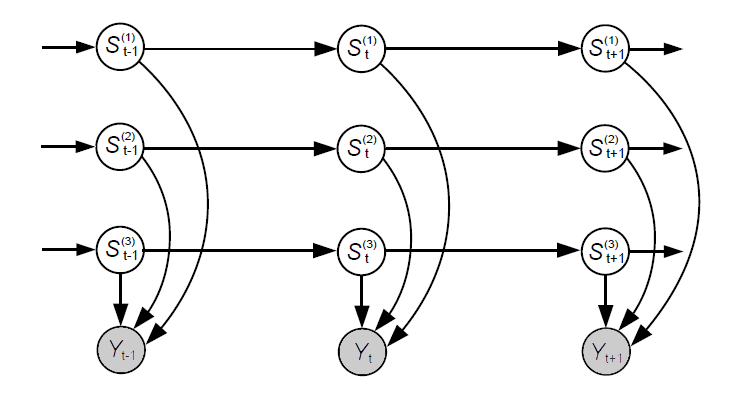
\includegraphics[width=0.8\textwidth]{billeder/FHMM.png}
\caption{Factorial hidden Markov model illustration. Source \citep{RefWorks:20}}
\label{fig:FHMM}
\end{figure}

As a extra constrain must each hidden state, in in each chain, only depended on the previously state in the chain, and not on the hidden state of other chains. This makes the state transition probability to be defined as in equation \ref{EQ:CTP}. 

\begin{equation}
	P(S_t|S_{t-1}) = \prod_{m = 1}^M P\left( S_t^{(m)}| S_{t-1}^{(m)} \right)
	\label{EQ:CTP}
\end{equation}

The observed stated is therefore created by the contribution of many different hidden states. 

In this implementation there is normally used only two or three states, since most appliances is seen as Type-I or Type-II appliances. There is trained one chain for each of the appliances plus one that is called the other chain. This chain is to allow for the other appliances that are not taken in to the model and noise. The model can therefore be used to validate for a given output what is the probability that a given appliance is contributing to the output. The concrete implementation for this algorithm has been borrowed from the \ab{NILMTK} \citep{RefWorks:21}. 

\subsection{Parson}
The Parson algorithem is a variant of the Kolter and Jaakkola algorithem\citep{RefWorks:22}. The algorithm is designed to be a semi-supervised learning algorithms. This means that the algorithm does not need to train on the data from the concrete house prior to deployment, but it still requires some prior knowledge. The idea is to have a database of general appliance models, that tells how specific appliances most likely will behave. This model will be able to detect the device, and do some unsupervised special training to better fit the concrete appliance. 

The algorithm is based on a kind of HMM called "difference HMM" since they take the step difference in the aggregated data and use as the observed output $Y_t$. In a normal \ab{HMM} there is only emitted one output for each hidden state in a chain. In the Parson algorithm the model is changed to output two states from the hidden states $X_t$ and $Y$. This creates a model structure that can be graphically illustrated as on figure \ref{Fig:ParsonModel}\citep{RefWorks:28}. 

\begin{figure}[H]
\begin{picture}(0,140)
\put(90,0){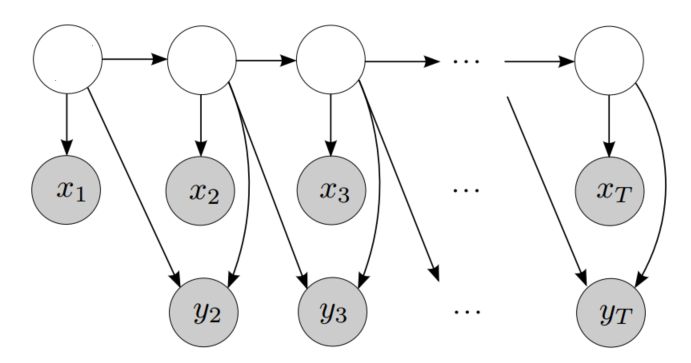
\includegraphics[width=0.6\textwidth]{billeder/ParsonIlu.png}}
\put(112,115){$S_1$}
\put(165,115){$S_2$}
\put(215,115){$S_3$}
\put(326,115){$S_T$}
\end{picture}
\caption{Parson hidden Markov model structure. Source \citep{RefWorks:28}}
\label{Fig:ParsonModel}
\end{figure}

The $Y_t$ is corresponding to the step in power that is observed since the last sample. It is assumed that the only thing that can cause a step in power is if an appliance changes states from one to another. The $X_t$ is the mean constant power draw of the state. This is used to filter out the appliance if the power draw observed is smaller than this threshold.

It is assumed that the power consumption of a state in the general model of an appliance can be modelled as a Gaussian. This can be illustrated as in equation \ref{EQ:GPF}. 

\begin{equation}
	w_t|_{S_t} \rightarrow \mathcal{N}( \mu_{S_t} , \sigma_{S_t}^2 )
	\label{EQ:GPF}
\end{equation}

This shows how the power draw of a appliance is modelled as Gaussians. The step Power $Y_t$, can also be modelled as a Gaussian that is created from the change between two states as shown in equation \ref{EQ:GST}.

\begin{equation}
	Y_t|_{S_t,S_{t-1}} \rightarrow \mathcal{N}( \mu_{S_t} - \mu_{S_{t-1}} , \sigma_{S_t}^2 + \sigma_{S_{t-1}}^2 )
	\label{EQ:GST}
\end{equation}

To model the constraint that the meter only can be on if the mean power draw is present in the signal is a additional constraint added to the emission probability. This constrain is mathematically described in equation \ref{EQ:PCA}.

\begin{equation}
	P(w_{S_t} \leq x_t | S_t ) = \int_{-\infty}^{x_t}  \mathcal{N}( \mu_{S_t} , \sigma_{S_t}^2 ) dw
	\label{EQ:PCA}
\end{equation}

Where $x_t$ is the measured power consumption and $w_{S_t}$ is the appliance power draw constraint. This makes the probobility going towards zero if the total power draw is to little and towards 1 if there is more than enough power. This is a loose constraint since too high power draw also could be created by other appliances. To minimise the impact this have for the algorithm is the mean power draw subtracted from the data before searching for other appliances. 

In the implementation validated in this paper are all appliances modelled as Type-I. The algorithm is allowed to train on the house data, to better fit the general models to the appliances and create the initial database.

\subsection{Weiss}
The algorithm proposed by Weiss called "AppliSense" is a other approach that do not use Markov models\citep{RefWorks:23}. The philosophy is that some appliances like lamps and kettles are purely resistive, where others like washing machines and air conditions are more inductive and some appliances like laptops are more capacitive. By measuring not only the power consumption, but also the amount of reactive power it is revealed if there is inductive or capacitive appliances.

The algorithm is supervised since it requires a signature database to be created prior to usage. The signature database consists of how the changes will be in reactive and real power for a specific device when it is turned on and off. In their paper the authors show a method where this database can be created of a user, by using a smart-phone application and turning on and off appliances in the house, and inputting the information in the mobile application\citep{RefWorks:23}. In this paper the database is created by data collected from the sub-meters measuring only the devices.  

The algorithm looks for significant power changes in the data. If a change is found it is assumed to be an on or off event. The change is now compared to all the values in the database. If a close match is found it is assumed to be this device, if not it is a unknown device. This limits the approach to Type-I appliances, and the algorithm requires the reactive power to be measured. 

\section{The ECO Dataset}
The experiments in this chapter will be done on the \ab{ECO}[Electricity Consumption and Occupancy] dataset \citep{RefWorks:26}\citep{RefWorks:27}. The dataset consists of six houses that have been equipped with sub-meters on selected meters and the main meter. The data is collected in Switzerland in the period June 2012 to January 2012. 

The data is sampled with a resolution on 1 Hz on both the sub-meters and the main meter. On the main meter is both real and reactive power measured, where on the sub-meter it is only the real power is measured. 

\begin{figure}[H]
\centering
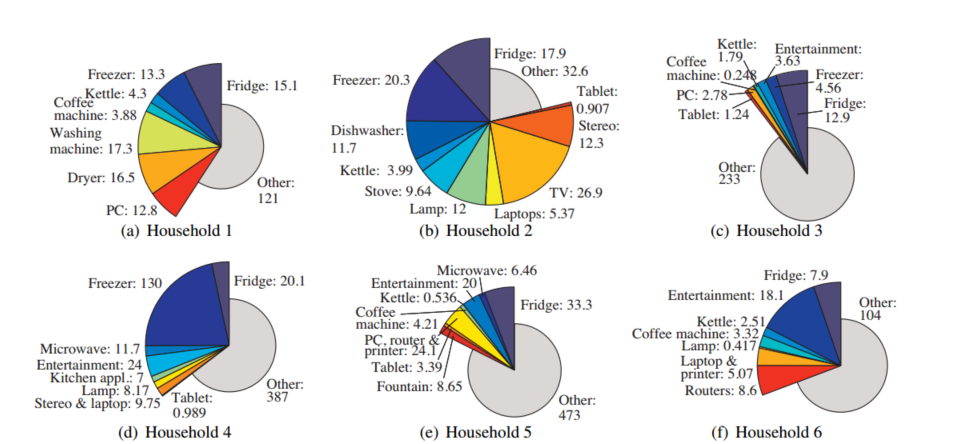
\includegraphics[width=1\textwidth]{billeder/ECOHouses.png}
\caption{House energy distribution. Source \citep{RefWorks:26}}
\label{fig:EHD}
\end{figure}

On figure \ref{fig:EHD} is shown how different appliances are responsible for the energy consumption in the different houses in the \ab{ECO} dataset. For house two more than $75\%$ of the energy usages is accounted for by the sub-meters. This makes house two a preferred candidate for experiments, since we know who the the heavy consumers are and who the little consumers are.  

\section{Validation of Methods} 
This section describes the experiments conducted using the three methods mentioned in section \ref{RecognitionMethods}. The experiments is validated using F1 and accuracy sensitivity and specificity metrics's. Since the focus is event detection a sample can fall in one of four categories. 

\begin{tabularx}{\linewidth}{ r X }
True Positive& This is when the guess says that there is an event, and there really is an event. Corresponding to the appliance is on. \\
\\
True Negative&This is when the guess says that there is no event, and there really is no event. Corresponding to when a appliance is turned off. \\
\\
False Positive& This is when the guess says that there is an event, but there really is no event. \\
\\
False Negative&This is when the guess says that there is no event, but there really is an event. \\\\
\end{tabularx}
The F1 and accuracy score is calculated as shown in equation \ref{EQ:F1} and \ref{EQ:ACC}

\begin{gather}
		TP = \text{number of true positives} \\
		TN = \text{number of true negatives} \\
		FP = \text{number of false positives} \\
		FN = \text{number of false negatives} \\
		recall = \frac{TP}{TP+FN} \label{EQ:recall}\\
		precision = \frac{TP}{TP+FP} \label{EQ:prec} \\
		F1 = 2 \times \frac{precision \times recall}{precision + recall} \label{EQ:F1}\\
		accuracy = \frac{TP+TN}{TN+TP+FN+FP} \label{EQ:ACC}
\end{gather}

The F1 score is mainly focused on how well the system guesses the the events, and do not score the true negatives. The accuracy is slightly different in that it looks at how many correct guesses there are in relation to the total amount of guesses. Fore a \ab{NILM} application the accuracy score on its own is not a very representative metric since some appliances have way more off time than on time. To guess that a appliance is off is just as good at guessing that it is on for the accuracy score. Appliances that are mostly off can therefore get a high accuracy score even though it is hard to determine when they are on. Therefore is it necessary also to look at the F1-score. This score tells how accurate it can be guessed when a appliance is on. This is done by combining the recall, that tells how many true positive was guess correctly in relation to the total amount of positives, as described by equation \ref{EQ:recall}, and the precision that is the ratio of correct guessed positives events in relation to all positive guesses, as shown on equation \ref{EQ:prec}. 

Five appliances have been selected from the \ab{ECO} dataset house 2. The appliances have been selected so there is some heavy and some little consumers. The appliances selected is: water kettle, fridge, TV, stereo and Laptop. All the methods will be traind using a training period of 15 days and validated on 75 days of data. 

\subsection{Sample rate experiment}
Common for the three methods is that they are designed for signals sampled at low sample rate. To determined the sensitivity, on the sample rate, is an experiment conducted where the dataset is downsampled to simulate different sample rates. The downsampling is done by applying a mean filter, so the new sample will be the average values of the samples in a specific period. This method is selected since it is the assumed behaviour of a meter that transmits samples at low rates. 

The results shown in figure \ref{fig:DSE} shows the average score of the different algorithms when recognising the five appliances. 

\begin{figure}[H]
\centering
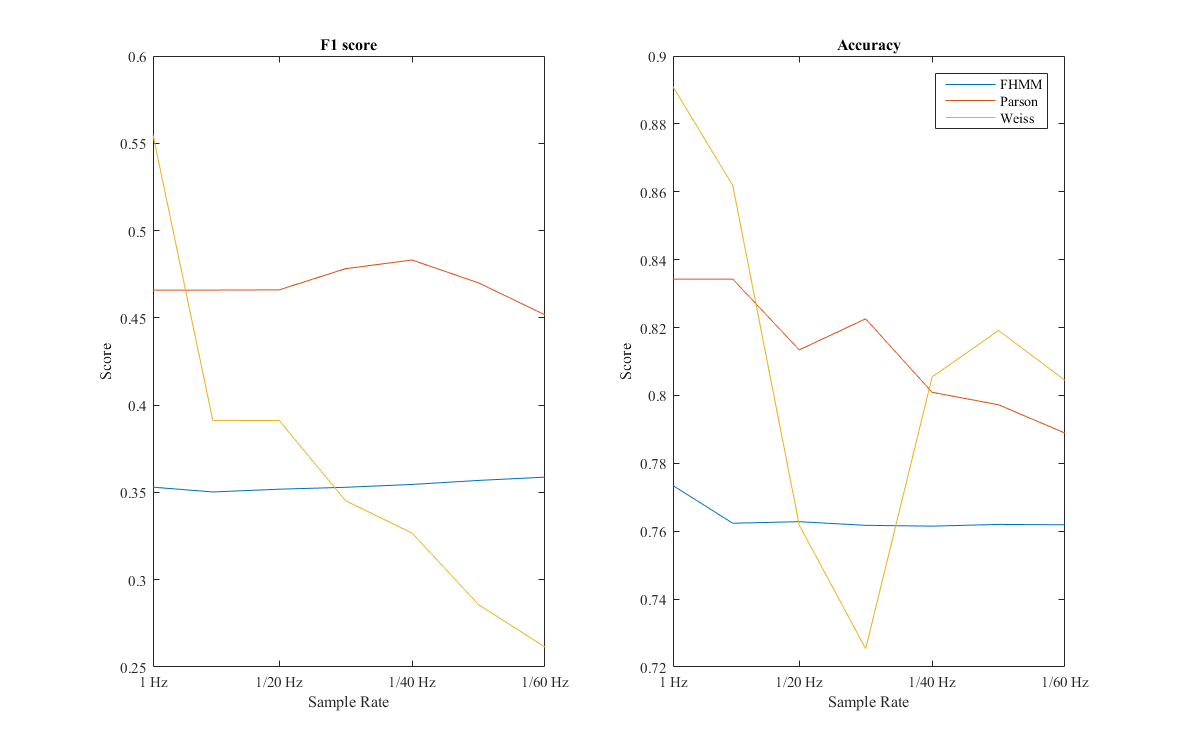
\includegraphics[width=1\textwidth]{billeder/AlgoScoreNilm.png}
\caption{Algorithm validation at different sample graduality.}
\label{fig:DSE}
\end{figure}

Both the accuracy and F1 score is shown. It is shown that for the Wiess clustering algorithms is the overall performance is decreasing for both scores. This indicates that is it both harder for it to determine when a appliance is on and when it is off. There is all most no change in the F1 score for the Parson and \ab{FHMM} algorithms that both builds on \ab{HMM}. Where the accuracy is decreasing for the parson as well. This tells that it finds the areas where the appliance is on just as well at high sample rate as for low. But to correctly guess the off periods is getting harder for the parson algorithm, where the \ab{FHMM} algorithm seems to be unaffected. 

It seems that for high sample rates does the Weiss algorithm preform superior to the others, where for lower is the Parson algorithm that preforms well. The \ab{FHMM} algorithm seems to preform worse that the others, but is more robust to changes in the sample rate. 

The results shown in figure \ref{fig:DSE} is the average for all appliances. The different appliances individual scores shows that some appliances is easier to find than others. The accuracy score for the different appliances is shown in figure \ref{fig:AccGS}. 

\begin{figure}[H]
\centering
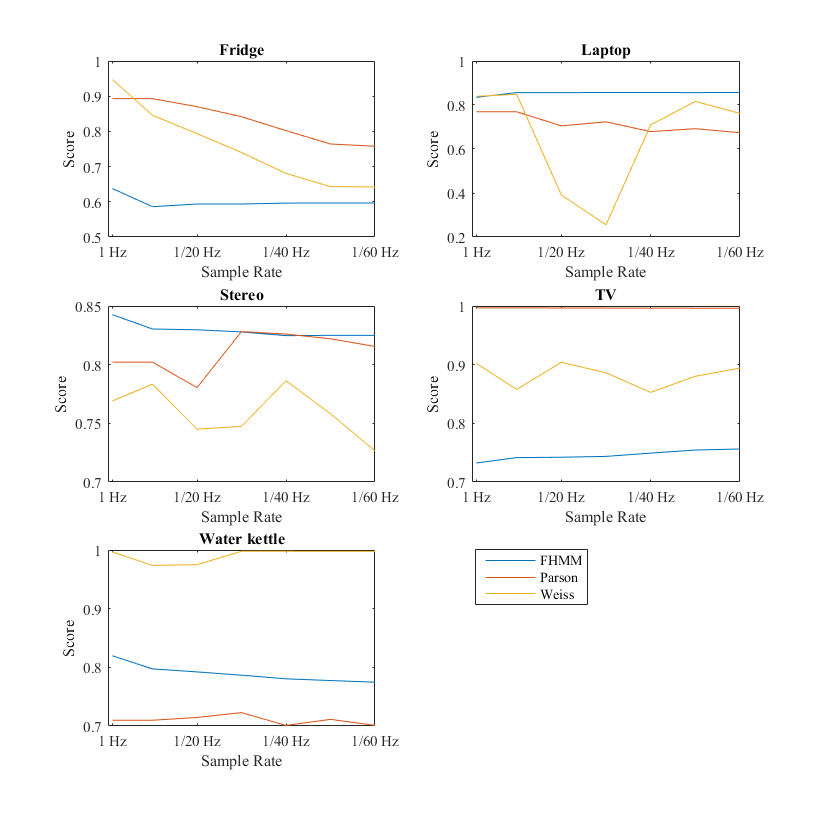
\includegraphics[width=0.8\textwidth]{billeder/App-AccuracyScore.png}
\caption{Appliances accuracy score}
\label{fig:AccGS}
\end{figure}

Since the accuracy score tells how well the all events are guessed it can be heavily dominated by the off events. Most of the appliances selected is mostly off appliances. Especially the water kettle is a good example as it is only used a few minuses each morning, and is off rest of the time. If it was assumed that this device was always off it would get a fairly high score since it is off most of the time.  

This is the reason why the score is fairly high for all the different appliances. It is also shown that the top algorithm is different form appliance to appliance. The fridge and the stereo is the only appliances that are greatly affected by the change in sample rate, the rest seems to be  relatively stable.

Since the accuracy score is dominated by the off periods, the F1 score is also shown in figure \ref{fig:AppF1}. This once again indicates how the different appliances has different algorithms that best detects them.  


\begin{figure}[H]
\centering
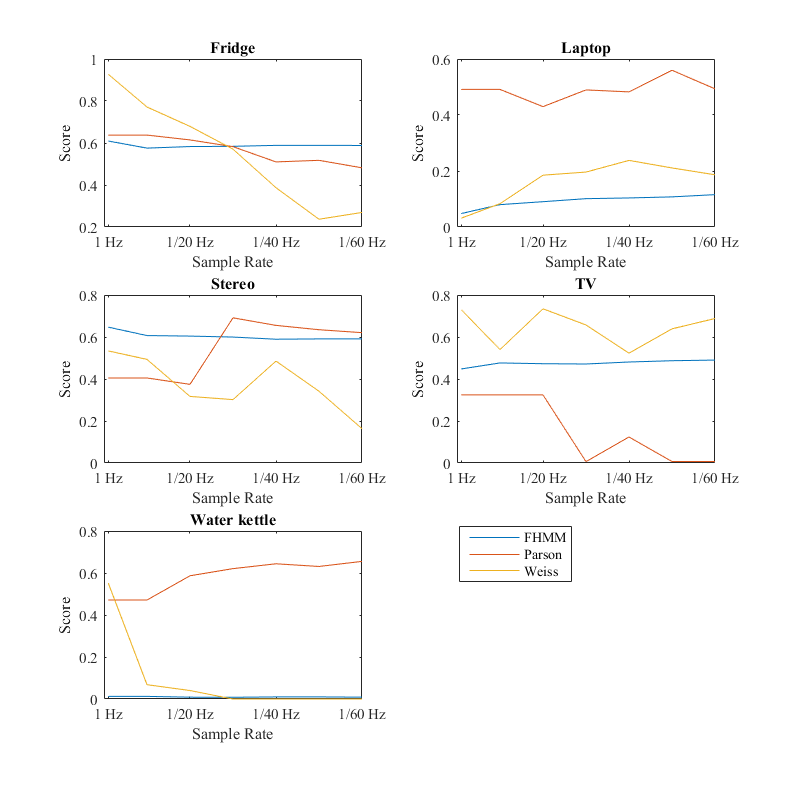
\includegraphics[width=0.8\textwidth]{billeder/App-F1Score.png}
\caption{Appliances F1 score}
\label{fig:AppF1}
\end{figure}

\newpage

\subsection{Error Tolerance Experiment}
\label{Sec:ETE}
As discussed in chapter \ref{Sec:DataQuality} is the data collected often filled with errors. This degrades the quality of the signal which can lead to worse performance. To validate the errors impact on the algorithms is a experiment conducted where the error rate is increased, and the F1 and accuracy score is measured. 

\begin{figure}[H]
\centering
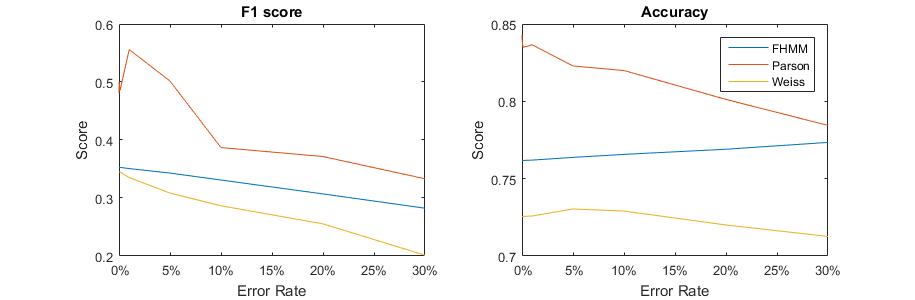
\includegraphics[width=1\textwidth]{billeder/AlgoErrorRate.png}
\caption{Algorithm validation at different error rate}
\label{fig:ErrorEx}
\end{figure}

The experiment was preformed by randomly introducing errors with a probability given by the error rate. This was done up to 30\% where approximately $\frac{1}{3}$ of the samples are missing. The results is shown in figure \ref{fig:ErrorEx}. It is shown that all methods is impacted by the errors, and have a decrease in performance. The experiment is conducted at a simulated sample rate on $\frac{1}{30} Hz$.

The algorithms tries as default to make a mean filtering to try to remove errors and noise. This will in situations with many errors remove some of the steps from the signal, and decrease the performance.  



\subsection{Gap Filling Experiment}
In chapter \ref{Sec:GapFill} it was described how mathematical gap filling methods could be used to estimate values for the missing gaps. It was mentioned that due to the stochastic nature of the signal, it was impossible to make a perfect reconstruction, but a qualifiedly guess could still be estimated.

In chapter \ref{Sec:GapFill} six methods of gap filling was evaluated. It turned out that the simple linear method preformed quite well in comparison to the others. The envelop method did also preform acceptable for smaller gaps. Therefore are these two method evaluated on the \ab{ECO} dataset, to see if it is possible to increase performance when preforming gap fixing. 


\begin{figure}[H]
\centering
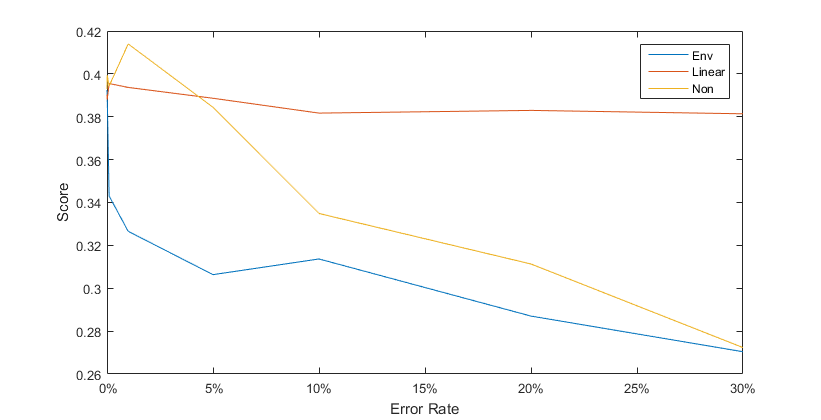
\includegraphics[width=1\textwidth]{billeder/EcoRecError.png}
\caption{Average recognition after recovery of the 3 methods}
\label{fig:GER}
\end{figure}

Like the error tolerance experiment described in section \ref{Sec:ETE}, is errors artificially introduced in the dataset. After this process is an attempt to removed the errors being done by using the gap filling techniques. 

On figure \ref{fig:GER} is the average F1 score shown for all 3 recognition methods applied on all 5 appliances. This indicates that by using a simple reconstruction method it is possible to keep the high performance. Where for the more advanced Envelope method seems to make it worse. This is typically because the more advanced types of reconstruction methods tries to model the frequency components, witch for greatly stochastic signals is more likely to introduce errors. 

To ensure that it is not one recognition method that courses the bad performance for the envelope is the results inspected for the individual appliances and methods. 


\newpage

\begin{figure}[H]
\centering
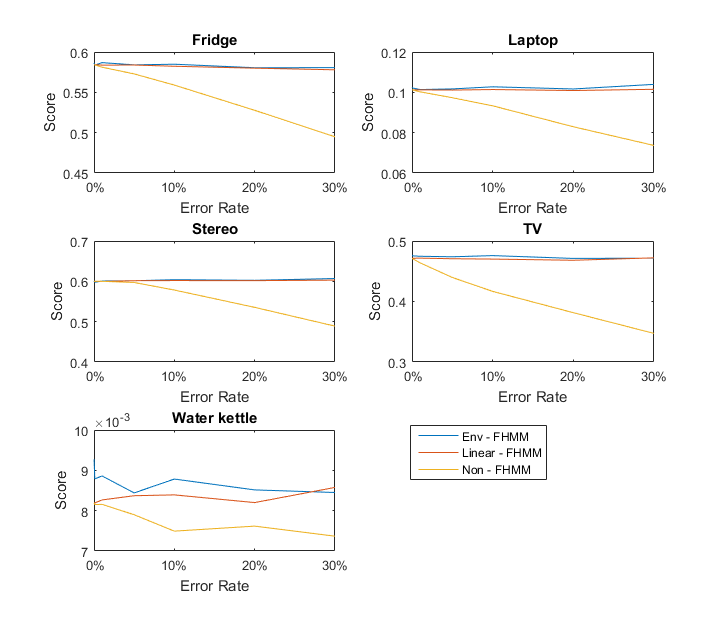
\includegraphics[width=1\textwidth]{billeder/Rec-FHMM.png}
\caption{Recovery in FHMM algorithm}
\label{fig:ERFHMM}
\end{figure}

On figure \ref{fig:ERFHMM} is the result from the reconstruction with the \ab{FHMM} algorithm shown. Here we see that the performance is prevented from decaying by the two reconstruction methods. It is also shown that the Envelope reconstruction actually preforms marginally better for the \ab{FHMM} algorithm. In all cases is the reconstruction better than non reconstruction. 

\newpage

\begin{figure}[H]
\centering
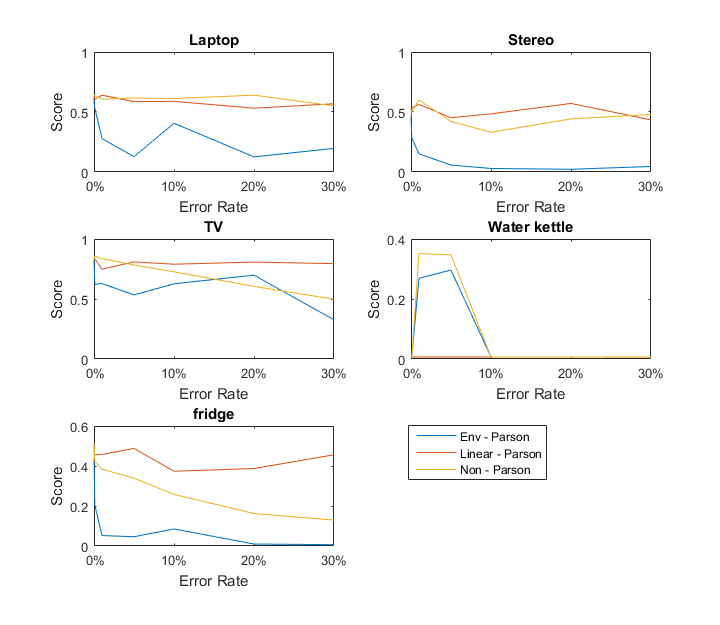
\includegraphics[width=1\textwidth]{billeder/Rec-Parson.png}
\caption{Recovery in Parson algorithm}
\label{fig:ERPARSON}
\end{figure}

On figure \ref{fig:ERPARSON} is the result from the reconstruction with the Parson algorithm shown. Here we see that the Envelope method is always worse than no reconstruction. For some of the appliances is the linear reconstruction a help, but fore some does it preform worse than no reconstruction. 

The parson algorithm does looks at jumps in the power, and usages a mean filter to only show the significant jumps. This behaviour can explains why a linear reconstruction gives almost no performance gain compared to no reconstruction for some of the devices.
 
\newpage
\begin{figure}[H]
\centering
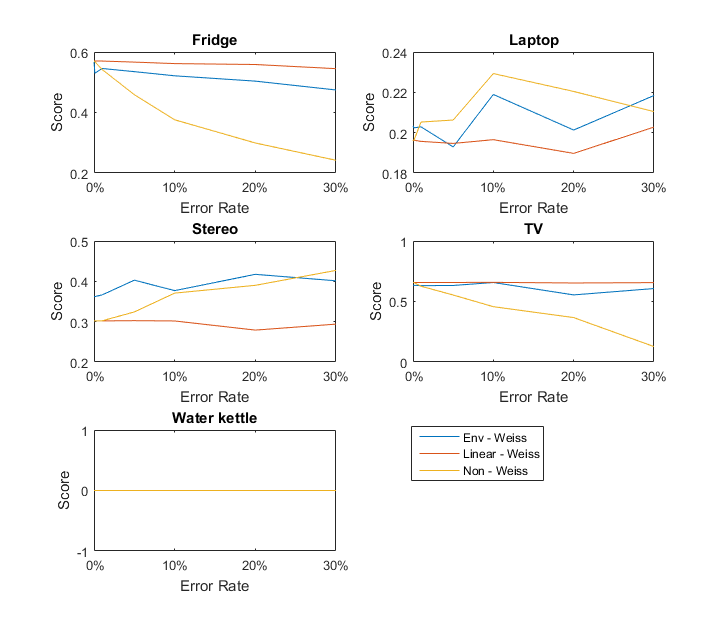
\includegraphics[width=1\textwidth]{billeder/Rec-Weiss.png}
\caption{Recovery in Weiss algorithm}
\label{fig:ERWEISS}
\end{figure}

On figure \ref{fig:ERWEISS} is the result from the reconstruction with the Weiss algorithm shown. For the Wiess algorithm it is appliance depended what reconstruction method is the best. Even though it seems like reconstruction is not preferred for some of the appliances like the laptop, is it worth noticing that the score is close to 0.2 which is a low score. For appliances that have a higher score like the TV and fridge reconstruction seems to work as intended.

The low score indicates that the method in it self is struggling to identify the appliance, and the data error is therefore not the primary problem.  